\subsection{Reducible configurations}

\begin{frame}
    \frametitle{Configurations}

    Configurations are planar graphs.

    \begin{definition}
        A configuration $\confg$ is \textit{contained} in a connected planar graph $G$ if $G\setminus \confg$ is connected.
    \end{definition}

    \begin{definition}
        A configuration $\confg$ is \emph{reducible} in a graph $G$ if its presence implies that the 4-coloring of $G$ can be reduced to the 4-coloring of $G'$ with less vertices.
    \end{definition}

    For the five color theorem, vertices of $\deg(v) \leq 5$ are all reducible configurations. Therefore we can always break down a 5-coloring problem.
\end{frame}

\begin{frame}
    \frametitle{Configurations}
    \begin{figure}
        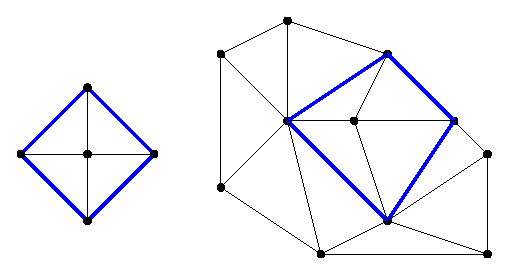
\includegraphics[width=0.8\textwidth]{images/contain1_good.eps}
    \end{figure}
\end{frame}

\begin{frame}
    \frametitle{Fundament of the Four Color Theorem}

    \begin{alertblock}{Four Color Theorem}
        Every planar graph $G$ strongly-contains a configuration $\confg$ that is either $k$-reducible, D-reducible or C-reducible in $G$.
    \end{alertblock}

    \begin{figure}
        \centering
        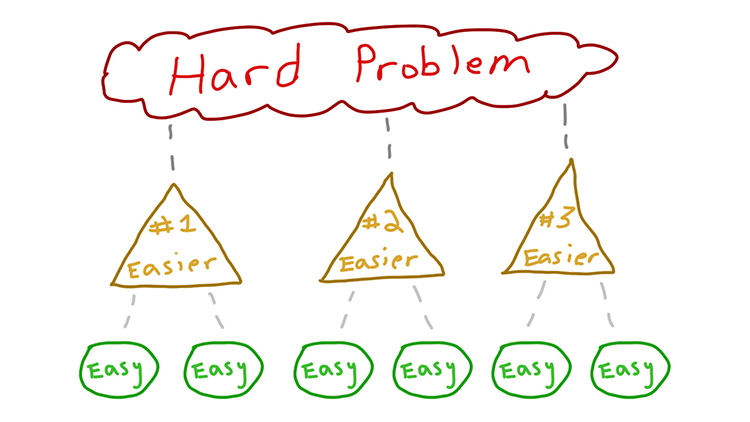
\includegraphics[width=0.7\textwidth]{images/breakdown.jpg}
    \end{figure}
\end{frame}